\chapter{Grundlagen}
In diesem Kapitel werden zunächst die wichtigsten Konzepte und Methode erläutert, die für das Verständnis von Systemen benötigt werden, an denen nur ein einzelner Agent beteiligt ist. Diese Systeme stellen einen sehr guten Einstiegspunkt für das weitere Verständnis dar und sollen die zugrundeliegenden Konzepte einfach und verständlich erläutern.
Diese werden anschließend vertieft und erweitert, sodass sie auf Systeme mit mehreren Agenten anwendbar werden. \\
Besonderer Fokus wird dabei auf das mathematische Verständnis gelegt, da im weiteren Verlauf der Arbeit vermehrt auf diese zurückgegriffen werden wird.

\section{Agenten}

In der Literatur gibt es keine eindeutige Definition für einen Agenten, allerdings existiert eine generelle Überschneidung dahingehend, dass ein intelligenter Agent alles sein kann, was seine Umgebung über Sensoren wahrnimmt und diese über Aktoren beeinflussen kann.
Um diese sehr generelle Beschreibung in ein konkretes Beispiel zu überführen, kann beispielhaft ein Roboter benutzt werden, dessen Aufgabe es ist, einen bestimmten Gegenstand anzuheben. Der Roboter nimmt seine Umgebung über eine Vielzahl von Sensoren wie \zB Kameras, Abstandsmesser oder ähnliches war. Diese Umgebung kann er \zB über einen oder mehrere Greifarme (Aktoren) beeinflussen. Der Roboter muss u.a. anhand der empfangenen Sensordaten die nächste Entscheidung treffen, um sein Ziel zu erreichen.
Abbildung \ref{fig:basics:agent} veranschaulicht das generelle Prinzip erneut anhand eines Flussdiagramms.
Im Verlauf dieser Arbeit wird neben der Anzahl und Komplexität der verschiedenen Aktoren auch die Größe und Wahrnehmbarkeit der Umgebung eine immer wichtigere Rolle bekommen,

\begin{itemize}
	\item da diese in ihrer Größe und Form nicht beschränkt ist. Die Umgebung kann \zB von der Größe eines Raumes bis hin zum gesamten Universum reichen.
	\item da die Umgebung häufig nicht vollständig von den Sensoren erfasst werden kann und der Agent so nur einen eingeschränkten Teil der Umgebung wahrnimmt.
\end{itemize}

\begin{figure}[ht!]
	\centering
	\scalebox{1.25}{	
\begin{tikzpicture}[
	node distance=7mm,
	title/.style={font=\fontsize{12}{14}\color{black!100}\ttfamily},
	box/.style={rectangle, draw=black!50, anchor=west}
	]
	%\node[title] (agent) {};
	
	%\node[box, below=of agent.east, xshift=5mm] (sensors) {Sensoren};
	\node[box] (sensors) {Sensoren};
	\node[draw=black!50, rectangle, below=of sensors] (magic) {Entscheidungslogik};
	\node[box, below=of magic] (acts) {Aktoren};
	\node [inner sep=10pt, minimum width=6cm, draw=black!50, fit={(sensors) (magic) (acts)}] (agent) {};
	\node[anchor=north west, title] at (agent.north west) {Agent};
	
	\node[draw=black!50, rectangle, right=of agent, inner sep=10pt] (env) {Umgebung};
	
	\draw[->] (sensors) -- (magic);
	\draw[->] (magic) -- (acts);
	
	\draw[->] (acts) -| (env) node[below left=1.3cm and 0.4cm, font=\small] (lbacts) {Aktion};
	\draw[->] (env) |- (sensors) node[above=2.6cm of lbacts, font=\small] {Auswerten};
\end{tikzpicture}
}
	\caption{Die Interaktion eines Agenten mit seiner Umgebung.}
	\label{fig:basics:agent}
\end{figure}
\todo{Entscheidungslogik richtig?}
\todo{Quellen, Grafik}

Wie in Abbildung \ref{fig:basics:agent} dargestellt ist, nimmt der Agent seine Übergebung über seine Sensoren war und versucht anhand dieser eine Handlungsentscheidung zu treffen. Diese Entscheidung wird anschließend in konkrete Aktionen übersetzt, die die Umgebung zum Vorteil des Agenten verändern sollen.
Welche konkrete Ausprägung die Entscheidungslogik dabei annimmt ist abhängig vom Aufbau und Typ des Agenten. \todo{Verweis auf weitere Quellen}

\section{Verhalten eines Agenten}
\label{chap:basics:behaviour}

Aufbauend auf der Definition eines Agenten und seinen Möglichkeiten, über Sensoren die Umgebung wahrzunehmen und durch Aktoren zu verändern, kann nun das Verhalten festgelegt werden. Durch jede Aktion, die der Agent durchführt, wird der Zustand seiner Umgebung auf eine bestimmte, eventuell unerwünschte Weise verändert. Anders als bei Menschen oder anderen Lebewesen, die ihre eigenen Ansichten und Vorstellung von einem erwünschten Endergebnis haben, ist dies bei Agenten nicht der Fall.
\todo{Erweitern}

Aus diesem Grund muss derjenige, der den Agenten und damit dessen eigentliches Ziel entwirft, besonders auf die korrekte Messung des Erfolges acht geben, denn dies kann mitunter eine große Herausforderung darstellen. 
Ob der Agent einen gewünschten Zustand durch eine Aktion erreicht hat, wird ihm entweder durch eine Belohnung (Reward) oder eine Bestrafung (Penalty) mitgeteilt. Im allgemeinen wird diese Bewertung auch als \textit{Performance Measure} bezeichnet und gibt dem Agenten ein entsprechendes Feedback, ob er durch sein Handeln einen gewünschten Zustand erreicht hat.
Ziel eines \textit{rationalen} Agenten ist es stets, die Summe seiner Belohnungen zu maximieren.  

Ein Agent, welcher \zB Schach spielt, könnte am Ende der Partie eine Belohnung von einem Punkt bekommen, bei einer Niederlage entsprechend einen Punkt abgezogen. Das Ziel des Agenten ist es in diesem Kontext, möglichst viele Partien zu gewinnen, um seine Belohnungen zu maximieren. 
Bei der Formulierung einen solchen Zieles kann mitunter der Fehler passieren, dass der Designer über die Belohnungen versucht, einen bestimmten \textit{Weg} vorzugeben, wie der Agent gewinnen soll. In diesem einfachen Beispiel kann es \zB eine zusätzliche Belohnung für das eliminieren der gegnerischen Dame geben, allerdings könnten bei diesem Vorgehen Probleme auftreten. Der Agent würde unter Umständen Wege finden, die Dame zu eliminieren, um eine bestimmte Belohnung zu bekommen, allerdings das übergeordnete Ziel - den Sieg der Partie - vernachlässigen.
%https://ai.stanford.edu/%7Eang/papers/icml04-apprentice.pdf

\todo{Erweitern: Agent entscheidet nur aufgrund der Sensoren oder auch mit vergangenem Wissen}

\section{Reinforcement Learning}

Das Reinforcement Learning stellt eine Reihe von Methoden zur Verfügung, damit ein Agent selbstständig lernen kann, wie er seinen akkumulierten Belohnungen maximiert. Dies ist besonders dann von großem Vorteil, wenn der Agent einer sich stetig ändernden, oder für ihn völlig unbekannten Umgebung ausgesetzt ist, da er sich selbstständig an die neuen Bedingungen anpassen kann. Die sehr abstrakte Belohnungs bzw. Bestrafungsmechanik aus Sektion \ref{chap:basics:behaviour} wird im folgenden konkretisiert und mathematisch beschrieben.
Die algorithmische Betrachtung des \textit{Lernens} für Agenten wird hingegen in Kapitel \ref{chap:learning} stark vertieft.

\subsection{\acf{MDP}}

Mithilfe des Markov-Entcheidungsprozesses ist es möglich, viele verschiedene Probleme des Reinforcement-Learning zu modellieren. Die generelle Funktionsweise des Prozesses ist in Abbildung \ref{fig.basics:rl:mdp} dargestellt.
Der Agent und die Umgebung (\textit{Environment}) interagieren zu bestimmten Zeitpunkten $t \in \mathbb{N}$ miteinander. In jeden Zeitpunkt $t$ teilt die Umgebung dem Agenten einen bestimmten Zustand $S_t \in \mathcal{S}$ mit, in dem diese sich gerade befindet.
$\mathcal{S}$ ist dabei die Menge aller möglichen Zustände.
Basierend auf dem erhaltenen Zustand führt der Agent anschließend die Aktion $A_t \in \mathcal{A}(S_t)$ aus, wobei $\mathcal{A}(S_t)$ für die Menge der möglichen Aktionen steht, die der Agent im Zustand $S_t$ ausführen kann.
Im darauffolgenden Zeitschritt $t + 1$ wird dem Agenten gleichzeitig mit der Belohnung bzw. Bestrafung $R_{t+1} \in \mathbb{R}$ der neuen Zustand $S_{t+1}$ der Umgebung mitgeteilt.

% https://commons.wikimedia.org/wiki/File:Markov_diagram_v2.svg
\begin{figure}[ht!]
	\centering
	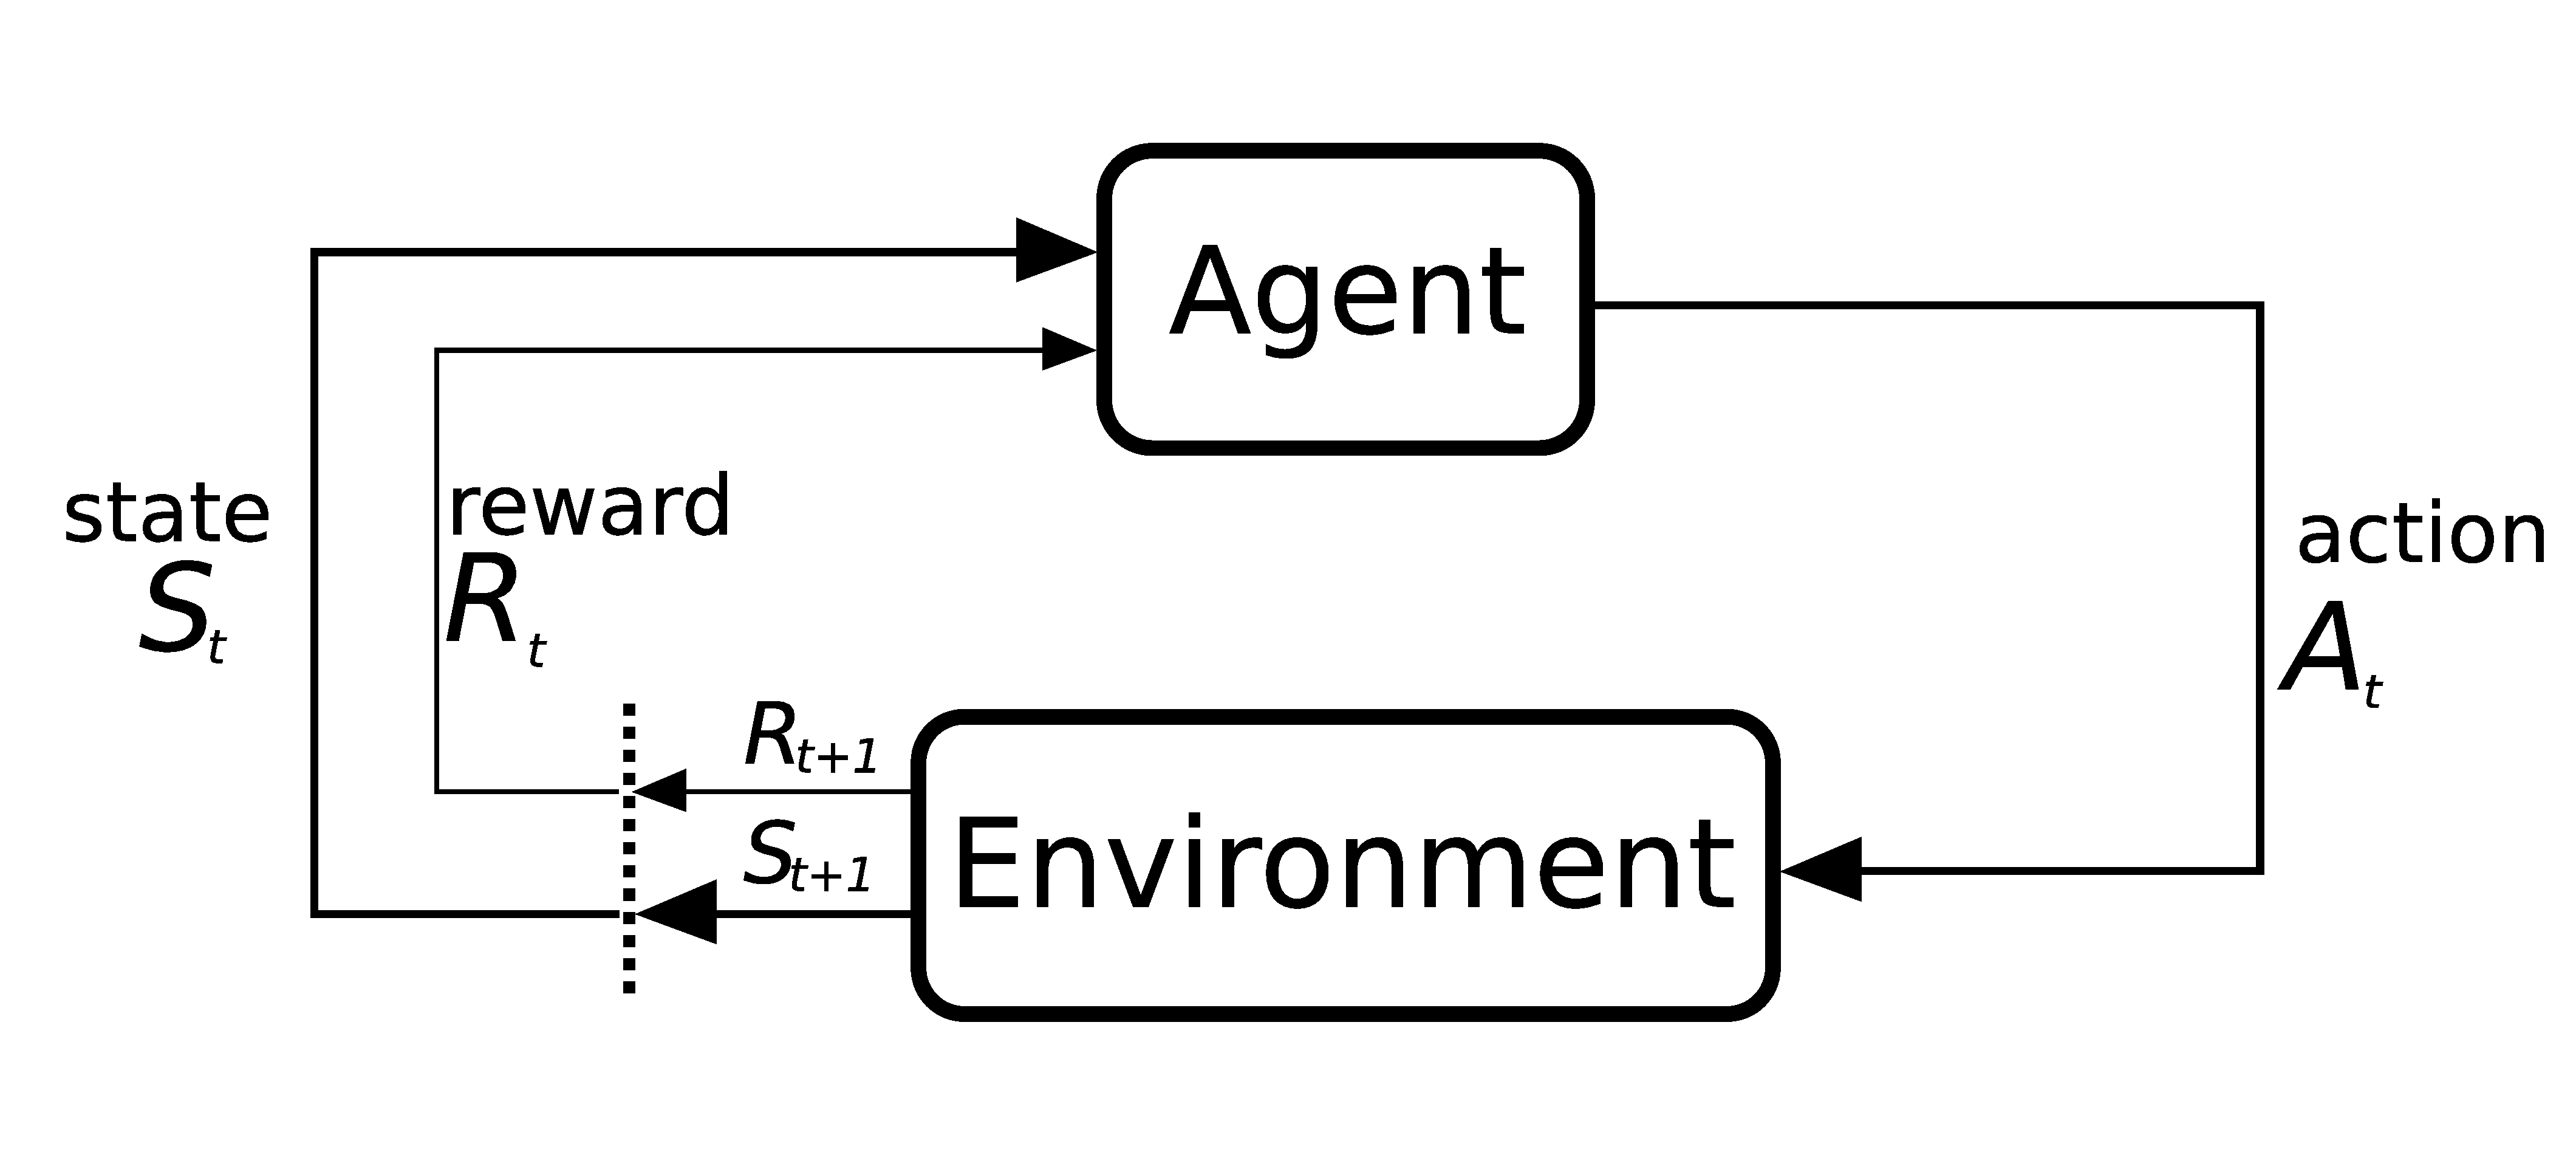
\includegraphics[scale=0.2]{Bilder/markov_diagram}
	\caption{Funktionsweise des Markov-Entscheidungsprozesses im Reinforcement Learning.}
	\label{fig.basics:rl:mdp}
\end{figure}

Die Entscheidung, welche Aktion in welchem Zustand ausgewählt wird, ist über die \textit{Policy} $\Pi_t$ des Agenten realisiert. $\Pi_t(a, s)$ ist dabei die Wahrscheinlichkeit, dass $A_t = a$, unter der Voraussetzung $S_t = s$. Vereinfacht ausgedrückt beschreibt $\Pi_t(a, s)$ damit die Wahrscheinlichkeit, dass zum Zeitpunkt $t$ im Zustand $s$ die Aktion $a$ gewählt wird.



\subsubsection{Markov-Eigenschaft}

Die Markov-Eigenschaft ist ein zentraler Bestandteil des \ac{MDP} und beschreibt 

\subsection{Bellman Gleichungen}

\section{}